%!TEX root = ../../Master.tex
\section{Organisation}

\subsection{ANF}

Aalborg/Nørresundby Fritidshavn er en paraplyorganisation for følgende sejlklubber. \cite{anf_havnereglement}
\begin{itemize}
	\item Aalborg Sejlklub
	\item Fiskerklyngen
	\item Vestre Baadelaug
	\item Sejlklubben Limfjorden
	\item Nørresundby Sejlklub
\end{itemize}
 
 Dette betyder at ANF forestår forhandlinger på vegne af organisationens sejlklubber. En fælles brugsaftale af nedenstådende havne, kan derved indgås med havneejer, Aalborg kommune.

 \begin{itemize}
 	\item Marina Fjordpark
 	\item Skudehavnen - lystbådehavnsafsnit
 	\item Vestre Baadehavn - lystbådehavnsafsnit
 	\item Nordre Baadehavn
 \end{itemize}

 ANF's indtægter består af bådpladsafgifter, som medlemsklubberne skal betale, for brug af de tilknyttede havne \cite{anf_budget_2013}. ANF forpligter sig til vedligeholdelse af havnene tilknyttet foreningen.

 \cite{anf_brugsaftale_2012}

 \begin{figure}
 	\begin{center}
 		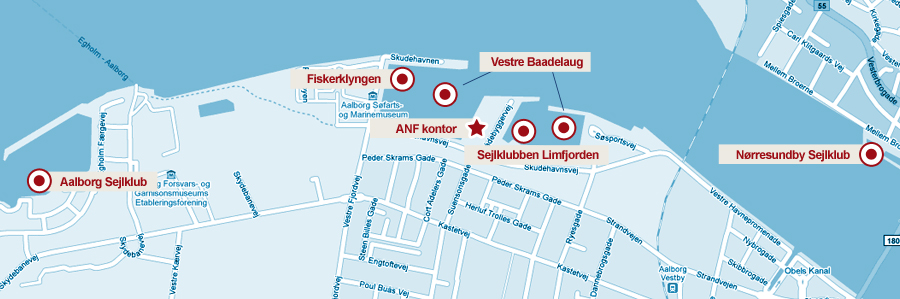
\includegraphics[width=\textwidth]{anf_overblik.jpg}
 	\end{center}
 	\caption{Overblik over medlemmerne af ANF}
 	\label{fig:anf_overblik}
 \end{figure}

\subsection{Bådklubber}

\subsubsection{Aalborg lystbådehavn}